The toggle visibility feature in the graphical interface allows users to
control the display of specific decompositions. This functionality proves
beneficial in various scenarios, such as when users want to concentrate solely
on a single decomposition, compare two decompositions side by side, or exclude
a discarded decomposition from the view. Without this feature, all selected
decompositions would remain in an active state, potentially cluttering the
visual interface. \Cref{fig:toggle_decomposition} showcases this toggle
visibility feature on and off states, enabling users to easily switch between
displaying or hiding specific decompositions according to their needs and
preferences.

\begin{figure*}[!htb]
  \centering
  \begin{subfigure}[!htb]{1\textwidth}
    \caption{Off State}
    \centering
    \begin{subfigure}[b]{0.49\textwidth}
      \centering
      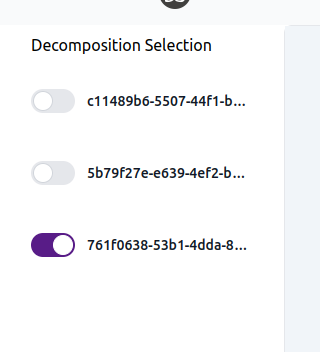
\includegraphics[width=\textwidth]{toggle_selection_off}
    \end{subfigure}
    \hspace{-0.1cm}
    \begin{subfigure}[b]{0.49\textwidth}
      \centering
      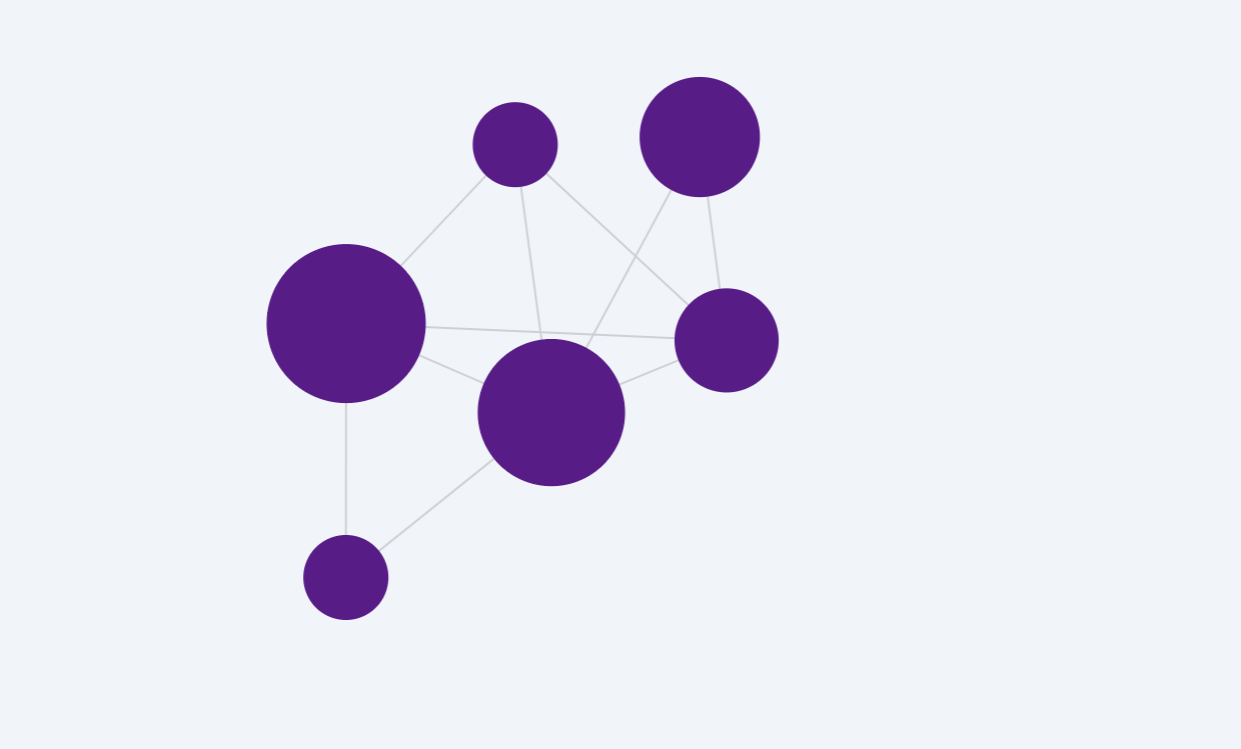
\includegraphics[width=\textwidth]{toggle_selection_off_graph}
    \end{subfigure}
  \end{subfigure}
  \hfill
  \begin{subfigure}[!htb]{1\textwidth}
    \caption{On State}
    \centering
    \begin{subfigure}[b]{0.49\textwidth}
      \centering
      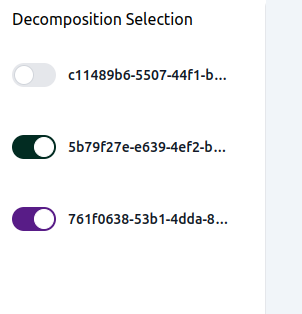
\includegraphics[width=\textwidth]{toggle_selection_on}
    \end{subfigure}
    \hspace{-0.1cm}
    \begin{subfigure}[b]{0.49\textwidth}
      \centering
      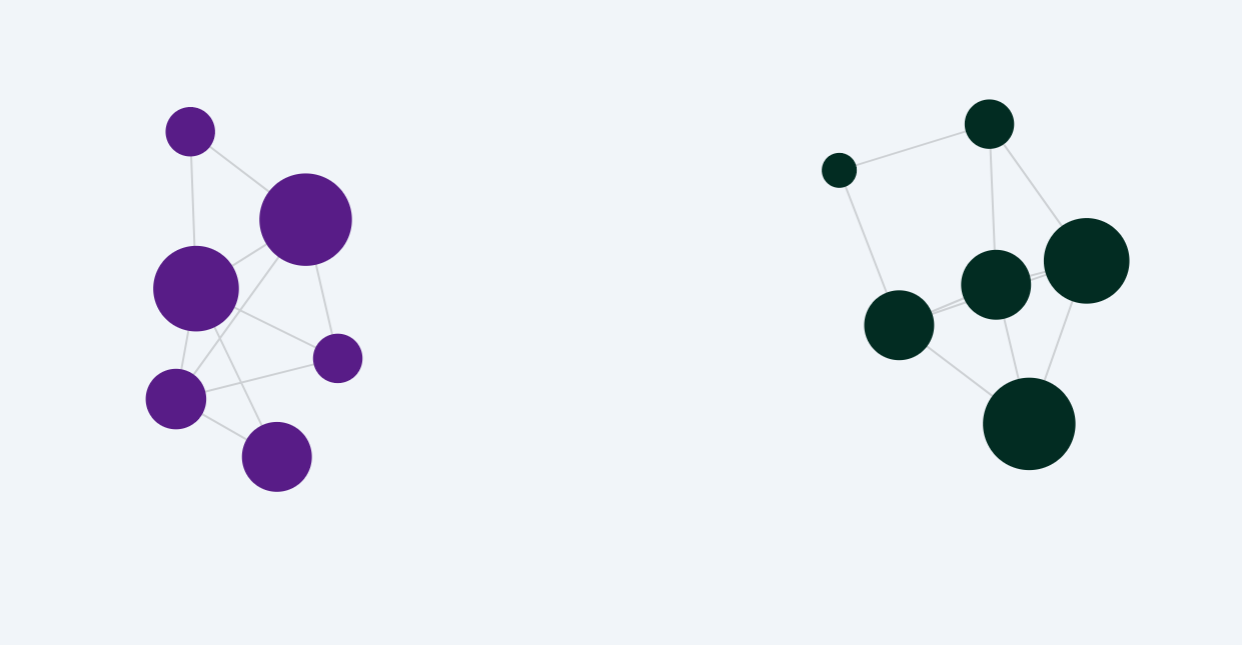
\includegraphics[width=\textwidth]{toggle_selection_on_graph}
    \end{subfigure}
  \end{subfigure}
  \caption{Toggle Decomposition}
  \label{fig:toggle_decomposition}
\end{figure*}
